\documentclass[12pt,addpoints]{article}
\usepackage[utf8]{inputenc}
\usepackage[dvipsnames]{xcolor}
%\usepackage[usenames]{color}
\usepackage{stmaryrd}
%\usepackage{array}
\usepackage{xfp}
\usepackage{fp}
\usepackage{pgf}
\usepackage{graphicx}
\usepackage{subfigure}
\usepackage{mathtools}
\usepackage[natbibapa]{apacite}
\bibliographystyle{apacite}
\graphicspath{ {images/} }
\usepackage{vmargin}
\usepackage{amsmath}
\usepackage{circuitikz}
\usepackage{tikz}
\usepackage{tocloft}
\usetikzlibrary{calc}
\usetikzlibrary{arrows}

\usepackage{pgfplots}
\pgfplotsset{compat=1.10}
\usepgfplotslibrary{fillbetween}
\usetikzlibrary{patterns}

\usepackage{units}
\usepackage{setspace}
\usepackage{multicol}
\usepackage{multirow}
\usepackage{colortbl}
\usepackage{array}
\usepackage{booktabs}
\usepackage{caption}
\usepackage{amssymb}
\usepackage{amsfonts}
\usepackage{amsthm}
\usepackage{amsmath,yhmath}
\usepackage{geometry}
%\usepackage{subcaption}
\usepackage{graphicx}
\usepackage[export]{adjustbox}
\usepackage[framemethod=tikz]{mdframed}
\usepackage{lipsum}
\usepackage{tcolorbox}
\usepackage{tocloft}
\usepackage{fancyhdr}
%\usepackage[colorlinks,citecolor=red]{hyperref}
%\usepackage{}
%\newtcolorbox{mybox2}{colback=red!5!white,colframe=red!75!black,width=0.85\textwidth}
\newtcolorbox{mybox2}[1]{colback=gray!5!white,colframe=cyan!75!black,fonttitle=\bfseries,title=#1}

\newtcolorbox{mybox3}[1]{colback=gray!5!white,colframe=Maroon!75!black,fonttitle=\bfseries,title=#1}

\newtcolorbox{mybox4}[1]{colback=gray!5!white,colframe=LimeGreen!75!black,fonttitle=\bfseries,title=#1}


\newcommand{\listequationsname}{\Large Lista de ecuaciones}
\newlistof{myequations}{equ}{\listequationsname}
\newcommand{\myequations}[1]{%
\addcontentsline{equ}{myequations}{Ecuación\hspace{0.3em}\protect\numberline{\theequation}#1}\par}
\setlength{\cftmyequationsnumwidth}{1.75em}
\setlength{\cftmyequationsindent}{1.5em}
\addtocontents{equ}{~\hfill\textbf{Página}\par}


\definecolor{mycolor}{rgb}{0.122, 0.435, 0.698}
%\captionsetup[table]{name=Tabla}
%\usepackage{bigstrut}
\setpapersize{A4}
\setmargins{2.5cm}       % margen izquierdo
{1.5cm}                        % margen superior
{16.5cm}                      % anchura del texto
{23.42cm}                    % altura del texto
{10pt}                           % altura de los encabezados
{1cm}                           % espacio entre el texto y los encabezados
{0pt}                             % altura del pie de página
{2cm}                           % espacio entre el texto y el pie de página
\usepackage{diagbox}
\usepackage{slashbox}
\usepackage{url}
\usepackage[framemethod=TikZ]{mdframed}
%Theorem
\newcounter{theo}[section] \setcounter{theo}{0}
\renewcommand{\thetheo}{\arabic{section}.\arabic{theo}}
\newenvironment{theo}[2][]{%
\refstepcounter{theo}%
\ifstrempty{#1}%
{\mdfsetup{%
frametitle={%
\tikz[baseline=(current bounding box.east),outer sep=0pt]
\node[anchor=east,rectangle,fill=blue!20]
{\strut Theorem~\thetheo};}}
}%
{\mdfsetup{%
frametitle={%
\tikz[baseline=(current bounding box.east),outer sep=0pt]
\node[anchor=east,rectangle,fill=blue!20]
{\strut  ~#1};}}%%%%%%%%%Theorem~\thetheo:
}%
\mdfsetup{innertopmargin=10pt,linecolor=blue!20,%
linewidth=2pt,topline=true,%
frametitleaboveskip=\dimexpr-\ht\strutbox\relax
}
\begin{mdframed}[]\relax%
\label{#2}}{\end{mdframed}}
%%%%%%%%%%%%%%%%%%%%%%%%%%%%%%

\newtheorem{defi}{Inciso}[subsection]
\renewcommand{\listfigurename}{Lista de Figuras}
\renewcommand{\listtablename}{Lista de Tablas}
\renewcommand{\baselinestretch}{1.5}
\renewcommand{\abstractname}{Resumen}
\renewcommand{\figurename}{Figura}
\renewcommand{\contentsname}{\underline{Contenido}}
\renewcommand{\tablename}{Tabla}
\renewcommand{\cftfigfont}{Figura }
\renewcommand{\cfttabfont}{Tabla }
\addtocontents{toc}{~\hfill\textbf{Página}\par}
\addtocontents{lot}{~\hfill\textbf{Página}\par}
\addtocontents{lof}{~\hfill\textbf{Página}\par}
\providecommand{\keywords}[1]
{
  \textbf{\text{Palabras clave: }} #1
}

\title{\textbf{``MEJORAMIENTO Y AMPLIACIÓN DEL SERVICIO DEPORTIVO DE PRÁCTICA RECREATIVA EN LA A.P.V. CRUZ CUNCA DEL DISTRITO DE SICUANI PROVINCIA DE CANCHIS, DEPARTAMENTO DE CUSCO''\\
CUI N° 2339483
}}
\author{MUNICIPALIDAD PROVINCIAL DE CANCHIS}
\date{Julio 06, 2002}
\usepackage[hidelinks]{hyperref}

\pagestyle{fancy}
\fancyhf{}
\rhead{
\includegraphics[width=20mm]{cas.PNG}}
\lhead{
\includegraphics[width=20mm]{logo.jpg}}
%\rfoot{Página\ \thepage\ de \numpages}
\lfoot{Realizado por Bach. \textit{Alexis Pompilla Yábar}}
\cfoot{}
\renewcommand{\headrulewidth}{0.4pt}
\renewcommand{\footrulewidth}{0.4pt}
\rfoot{Página\ \thepage}
%\AtBeginDocument{\addtocontents{toc}{\protect\thispagestyle{empty}}} 
\begin{document}
%\setlength{\abovedisplayskip}{0pt}
%\setlength{\belowdisplayskip}{0pt}
%\setlength{\abovedisplayshortskip}{0pt}
%\setlength{\belowdisplayshortskip}{0pt}
\maketitle
\begin{figure}[h!]
    \centering
    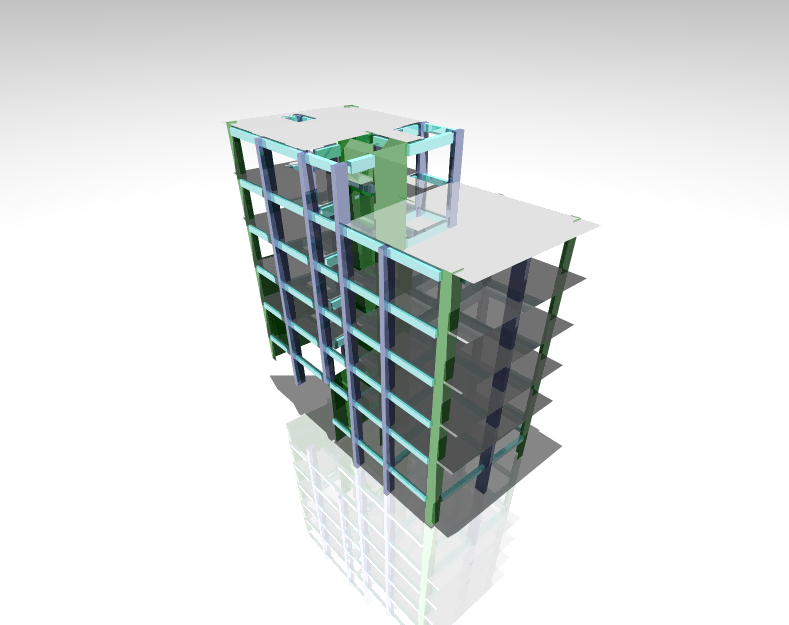
\includegraphics[scale=0.75]{IMAGENES/r2.png}
    \label{fig:my_label}
\end{figure}
\thispagestyle{empty}
\newpage

\clearpage                       % Otherwise \pagestyle affects the previous page.
{                                % Enclosed in braces so that re-definition is temporary.
  \pagestyle{empty}              % Removes numbers from middle pages.
  \fancypagestyle{plain}         % Re-definition removes numbers from first page.
  {
    \fancyhf{}%                       % Clear all header and footer fields.
    \renewcommand{\headrulewidth}{0pt}% Clear rules (remove these two lines if not desired).
    \renewcommand{\footrulewidth}{0pt}%
  }
    \begin{spacing}{1.35}
    \tableofcontents
  \end{spacing}
  \thispagestyle{empty}  
  \listoffigures
\newpage
\listoftables
  \thispagestyle{empty} 
% Removes numbers from last page.
}


%\listofmyequations
%\header{Realizado por: Alexis Pompilla Yábar}{}{}
\newpage
%\begin{abstract}
\thispagestyle{empty}
El presente documento contempla todo lo concerniente al análisis y diseño estructural de la vivienda multifamiliar para acciones gravitacionales y sísmicas según lo establecido en el reglamento nacional de edificaciones vigente. De manera preliminar se presentan los datos de la edificación como la ubicación, planta y elevación arquitectónica, resultados y recomendaciones del estudio de mecánica de suelos. Posterior a esto se realiza la estructuración y el predimensionamiento de los elementos estructurales siguiendo lo establecido en las normas y recomendaciones de especialistas en la rama. Finalmente se realiza el análisis sísmico según la norma E-030, se verifica las irregularidades y se construye el espectro de respuesta de aceleraciones que representa la demanda sísmica, se realiza el análisis modal y se determina las dimensiones finales de los elementos para dotar al edificio de suficiente rigidez lateral para cumplir la deriva máxima permisible en estructuras de concreto armado, finalmente se verifica el sistema estructural y se escala las fuerzas obtenidas con el análisis dinámico modal espectral al porcentaje mínimo respecto a la cortante basal estática para combinar las fuerzas con las acciones gravitacionales según lo establecido en la norma E-060. La estructura resultante consiste en un sistema estructural de muros en la dirección X y de pórticos en la dirección Y, y derivas máximas de aproximadamente 0,0035 en la dirección X y 0.006 en Y. Finalmente se muestra el diseño por resistencia ultima de los elementos de concreto armado que conforma la edificación.
\vfill
\begin{flushleft}
\keywords{Vivienda multifamiliar, Análisis sísmico, E-030, E-060.}
\end{flushleft}

\end{abstract}
\newpage
\pagenumbering{arabic}


\clearpage
\bibliography{biblio}
\end{document}

